\documentclass[10pt]{mypackage}

% sans serif font:
%\usepackage{cmbright}
%\usepackage{sfmath}
%\usepackage{bbold} %better blackboard bold

%serif font + different blackboard bold for serif font
\usepackage{newpxtext,eulerpx}
\renewcommand*{\mathbb}[1]{\varmathbb{#1}}

\usetikzlibrary{angles, quotes, intersections}
\usetikzlibrary{bending} % for arrow head angle
%\contourlength{1.0pt}
\usetikzlibrary{3d}

\usepackage[outline]{contour} % glow around text
\tikzset{>=latex} % for LaTeX arrow head

\colorlet{myblue}{blue!65!black}
\colorlet{mydarkblue}{blue!50!black}
\colorlet{myred}{red!65!black}
\colorlet{mydarkred}{red!40!black}
\colorlet{veccol}{green!70!black}
\colorlet{vcol}{green!70!black}
\colorlet{xcol}{blue!85!black}
%\colorlet{projcol}{xcol!60}
%\colorlet{unitcol}{xcol!60!black!85}
%\colorlet{myred}{red!90!black}
%\colorlet{mypurple}{blue!50!red!80!black!80}
\tikzstyle{vector}=[->,very thick,xcol,line cap=round]
\tikzstyle{xline}=[myblue,very thick]
\tikzstyle{yzp}=[canvas is zy plane at x=0]
\tikzstyle{xzp}=[canvas is xz plane at y=0]
\tikzstyle{xyp}=[canvas is xy plane at z=0]
\def\tick#1#2{\draw[thick] (#1) ++ (#2:0.12) --++ (#2-180:0.24)}
\def\N{100}
\tikzset{axis/.style={thick,-latex}}
\tikzset{vec/.style={thick,blue}}
\tikzset{univec/.style={thick,red,-latex}}
%Notation
\usepackage{physics}

\fancyhf{}
\rhead{Avinash Iyer}
\lhead{Mathematical Methods of Physics: Class Notes}

\setcounter{secnumdepth}{0}

\begin{document}
\section{Things You Just Gotta Know}%
\subsection{Coordinate Systems}%
We want to focus on vector-valued functions of coordinates.
\begin{align*}
  \vec{V}(\mathbf{r}) &= V_x(x,y)\hat{i} + V_y(x,y)\hat{j}.
\end{align*}
Notice that a vector function uses the coordinate system twice. Once for the function's inputs, once for the vectors themselves.
\subsubsection{Polar Coordinates}%
\begin{center}
  %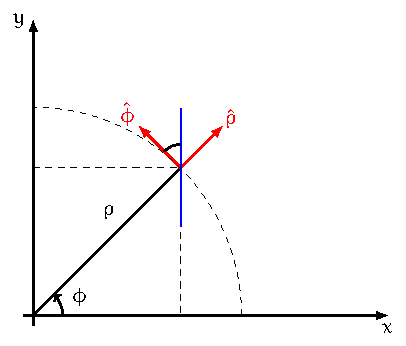
\includegraphics[width=10cm]{polar_coordinates.pdf}
	\begin{tikzpicture}
%		%Grid
%		\draw[thin, dotted] (0,0) grid (8,8);
%		\foreach \i in {1,...,8}
%		{
%			\node at (\i,-2ex) {\i};	
%		}
%		\foreach \i in {1,...,8}
%		{
%			\node at (-2ex,\i) {\i};	
%		}
%		\node at (-2ex,-2ex) {0};
		
		%Coordinates		
		\coordinate (A) at (6,0);
		\coordinate (B) at (0,0);
		\coordinate (C) at (2.5,2.5);
		\coordinate (B') at (2.5,3.5);
		\coordinate (A') at (1.8,3.2);
		
		%Axis
		\draw[thick,-latex] (-1ex,0) -- (6,0) node [below] {$x$};
		\draw[thick,-latex] (0,-1ex) -- (0,5) node [left] {$y$};
		
		%Vectors
		\draw[thick] (0,0) -- (2.5,2.5) node[pos=0.6, above left] {$\rho$};
		\draw[thick, red, -latex] (2.5,2.5) -- (3.2,3.2) node[pos=1.2] {$\hat{\rho}$};
		\draw[thick, red, -latex] (2.5,2.5) -- (1.8,3.2) node[pos=1.3] {$\hat{\phi}$};
		
		%Help Lines
		\draw[dashed] (0,2.5) -- (2.5,2.5) -- (2.5,0);
		\draw[blue, thick] (2.5,3.5) -- (2.5,1.5);
		\draw[dashed] (3.53,0) arc (0:90:3.53);
		
		%Angle
		\pic[draw, ->, thick, "$\phi$", angle eccentricity=1.7] {angle = A--B--C};
		\pic[draw, thick, angle radius=4mm, angle eccentricity=1.7] {angle = B'--C--A'};
		
	\end{tikzpicture}
\end{center}
We can also express the inputs to $ \vec{V} $ in polar coordinates, $(\rho,\phi)$.
\begin{align*}
  \vec{V}(\mathbf{r}) &= V_{\rho}\left(\rho,\phi\right)\hat{i} + V_{\phi}\left(\rho,\phi\right)\hat{j}.
\end{align*}
To extract the input functions, we take
\begin{align*}
  V_x &= \hat{i}\cdot \vec{V}\\
  V_y &= \hat{j}\cdot \vec{V}.
\end{align*}
Alternatively, we can project $ \vec{V} $ onto the $\hat\rho,\hat\phi$ axis:
\begin{align*}
  \vec{V}(\mathbf{r}) &= V_{\rho}\left(\rho,\phi\right)\hat{\rho} + V_{\phi}\left(\rho,\phi\right)\hat{\phi},
\end{align*}
and we extract
\begin{align*}
  V_{\rho} &= \hat{\rho}\cdot \vec{V}\\
  V_{\phi} &= \hat{\phi}\cdot \vec{V}.
\end{align*}
Notice that $\mathbf{r}$ is an abstract vector; we need to project it onto a basis.\newline

For instance, we can take the position vector and project it onto the cartesian and polar axes:
\begin{align*}
  \mathbf{s} &= x\hat{i} + y\hat{j}\\
             &= \rho \cos \phi \hat{i} + \rho \sin \phi \hat{j}\\
             &= \rho \hat{\rho}\\
             &= \sqrt{x^2 + y^2}\hat{\rho}
\end{align*}
The main reason we avoided using the $\hat\rho,\hat\phi$ axis up until this point is that $\rho$ and $\phi$ are \textit{position-dependent}, while the $\hat{i},\hat{j}$ axis is position-independent.\newline

Now, we must figure out the position-dependence of $\hat{\rho}$ and $\hat{\phi}$:
\begin{align*}
  d\mathbf{r} &= \pd{\mathbf{r}}{\rho}d\rho + \pd{\mathbf{r}}{\phi}d\phi.
\end{align*}
If we hold $\phi$ constant, it must be the case that any change in $\rho$ is in the $\hat\rho$ direction. Therefore,
\begin{align*}
  \hat\rho &= \frac{\pd{\mathbf{r}}{\rho}}{\left\Vert \pd{\mathbf{r}}{\rho} \right\Vert}\\
           &= \frac{\cos\phi\hat{i} + \sin\phi\hat{j}}{\left\vert \cos\phi\hat{i} + \sin\phi\hat{j} \right\vert}\\
           &= \cos\phi\hat{i} + \sin\phi\hat{j}.
\end{align*}
Similarly,
\begin{align*}
  \hat\phi &= \frac{\pd{\mathbf{r}}{\phi}}{\norm{\pd{\mathbf{r}}{\rho}}}\\
           &= \frac{-\rho\sin\phi\hat{i} + \rho\cos\phi\hat{j}}{\left\Vert -\rho\sin\phi\hat{i} + \rho\cos\phi\hat{j} \right\Vert}\\
           &= -\sin\phi\hat{i} + \cos\phi\hat{j}.
\end{align*}
Thus, we can see that the $\hat\rho,\hat,\phi$ axis is orthogonal. 
\begin{align*}
  \pd{\hat{\rho}}{\phi} &= -\sin\phi\hat{i} + \cos\phi\hat{j}\\
                        &= \hat{\phi},\\
  \pd{\hat{\phi}}{\phi} &= -\hat{\rho},\\
  \pd{\hat{\phi}}{\rho} &= 0,
  \intertext{and}
  \pd{\hat{\rho}}{\rho} &= 0
\end{align*}
\begin{example}[Velocity]
  \begin{align*}
    \mathbf{v} &= \frac{d \mathbf{s}}{dt}\\
               &= \frac{d}{dt}\left(x\hat{i}\right) + \frac{d}{dt}\left(y\hat{j}\right).
               \intertext{In the case of cartesian coordinates, $\hat{i}$ and $\hat{j}$ are constants.}
               &= v_{x}\hat{i} + v_{y}\hat{j}
  \end{align*}
  When we examine polar coordinates, since $\hat{\rho}$ and $\hat{\phi}$ are position-dependent, we must use the chain rule.\footnote{Note that $\hat{\rho} = \hat{\rho}\left(\rho,\phi\right)$ and $\hat{\phi} = \hat{\phi}(\rho,\phi)$.}
  \begin{align*}
    \mathbf{v} &= \frac{d\mathbf{s}}{dt}\\
               &= \frac{d\rho}{dt}\hat{\rho} + \rho \frac{d\hat{\rho}}{dt}\\
               &= \frac{d\rho}{dt}\hat{\rho} + \rho \left(\cancelto{0}{\pd{\hat{\rho}}{\rho}}\frac{d\rho}{dt} + \underbrace{\pd{\hat{\rho}}{\phi}}_{=\hat{\phi}}\frac{d\phi}{dt}\right)\\
               &= \frac{d\rho}{dt}\hat{\rho} + \rho \frac{d\phi}{dt}\hat{\phi}\\
               &= \dot\rho\hat\rho + \rho\dot\phi\hat\phi.
  \end{align*}
  Notice that $\dot\rho$ is the radial velocity and $\dot\phi = \omega$ is the angular velocity.
\end{example}
\subsubsection{Spherical and Cylindrical Coordinates}%
\begin{center}
  %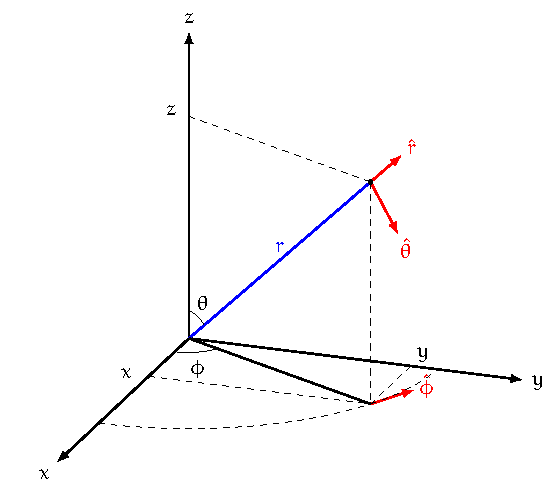
\includegraphics[width=10cm]{spherical_coordinates.pdf}

	\tdplotsetmaincoords{70}{110}
	%
	\pgfmathsetmacro{\thetavec}{48.17}
	\pgfmathsetmacro{\phivec}{63.5}
	%
	
	\begin{tikzpicture}[tdplot_main_coords]
		%Axis
		\draw[axis] (0,0,0) -- (6.5,0,0) node [pos=1.1] {$x$};
		\draw[axis] (0,0,0) -- (0,6,0) node [pos=1.05] {$y$};
		\draw[axis] (0,0,0) -- (0,0,5.5)  node [pos=1.05] {$z$};   
		
		%Unit Vectors
%		\tdplotsetcoord{p}{1}{90}{\phivec}
%    	\draw[univec] (2,4,0) -- ($(p)+(2,4,0)$) node [pos=1.35] {$\vu*{\varpi}$};
		\tdplotsetcoord{P'}{7}{\thetavec}{\phivec}
    	\draw[univec] (0,0,0) -- (P') node [pos=1.05] {$\hat{r}$};
    	\tdplotsetcoord{P''}{1}{90}{90+\phivec}
    	\draw[univec] (2,4,0) -- ($(P'') + (2,4,0)$) node [pos=1.3] {$\hat{\phi}$};
    	\tdplotsetcoord{P'''}{1}{90+\thetavec}{\phivec}
    	\draw[univec] (2,4,4) -- ($(P''') + (2,4,4)$) node [pos=1.3] {$\hat{\theta}$};
		
		%Vectors
		\tdplotsetcoord{P}{6}{\thetavec}{\phivec}
		\draw[vec] (0,0,0) -- (P) node [midway, above] {$r$};
		\draw[thick] (0,0,0) -- (2,4,0);
		
		%Help Lines
		\draw[dashed] (2,4,4) -- (2,4,0);
		\draw[dashed] (2,0,0) -- (2,4,0) node [pos=-0.1] {$x$};
		\draw[dashed] (0,4,0) -- (2,4,0) node [pos=-0.3] {$y$};
		\draw[dashed] (0,0,4) -- (2,4,4) node [pos=-0.1] {$z$};
		\draw[dashed, tdplot_main_coords] (4.47,0,0) arc (0:90:4.47);
		
		%Point
		\node[fill=black, circle, inner sep=0.8pt] at (2,4,4) {};
		
		%Angles
		\tdplotdrawarc{(0,0,0)}{0.7}{0}{\phivec}{below}{$\phi$}
		 
	    \tdplotsetthetaplanecoords{\phivec}
	    \tdplotdrawarc[tdplot_rotated_coords]{(0,0,0)}{0.5}{0}{\thetavec}{}{}
	    \node at (0,0.25,0.67) {$\theta$};
		
	\end{tikzpicture}
\end{center}
\begin{center}
  	\tdplotsetmaincoords{70}{110}
	%
	\pgfmathsetmacro{\thetavec}{48.17}
	\pgfmathsetmacro{\phivec}{63.5}
	%
	
	\begin{tikzpicture}[tdplot_main_coords]
		%Axis
		\draw[axis] (0,0,0) -- (6,0,0) node [pos=1.1] {$x$};
		\draw[axis] (0,0,0) -- (0,6,0) node [pos=1.05] {$y$};
		\draw[axis] (0,0,0) -- (0,0,5.5)  node [pos=1.05] {$z$};   
		
		%Help Lines
		\draw[dashed] (2,4,4) -- (2,4,0);
		\draw[dashed] (2,0,0) -- (2,4,0) node [pos=-0.1] {$x$};
		\draw[dashed] (0,4,0) -- (2,4,0) node [pos=-0.35, left] {$y$};
		\draw[dashed] (0,0,4) -- (2,4,4) node [pos=-0.1] {$z$};
		\draw[dashed, tdplot_main_coords] (4.47,0,0) arc (0:90:4.47);
		
		%Unit Vectors
		\tdplotsetcoord{P'}{1}{90}{\phivec}
    	\draw[univec] (2,4,0) -- ($(P')+(2,4,0)$) node [pos=1.3] {$\hat{\rho}$};
    	\tdplotsetcoord{P''}{1}{90}{90+\phivec}
    	\draw[univec] (2,4,0) -- ($(P'') + (2,4,0)$) node [pos=1.3] {$\hat{\phi}$};
    	
    	%Vectors
		\tdplotsetcoord{P}{6}{\thetavec}{\phivec}
		\draw[vec] (0,0,0) -- (P);
		\draw[thick] (0,0,0) -- (2,4,0) node [pos=0.6, above] {$\rho$};
		
		%Point
		\node[fill=black, circle, inner sep=0.8pt] at (2,4,4) {};
		
		%Angles
		\tdplotdrawarc{(0,0,0)}{0.7}{0}{\phivec}{below}{$\phi$}
		
	\end{tikzpicture}
\end{center}
\begin{center}
  \renewcommand{\arraystretch}{1.5}
  \begin{tabular}{c|c|c}
    Polar & Cylindrical & Spherical\\
    \hline
    $\mathbf{s} = s(\rho,\phi)$ & $\mathbf{s} = s(\rho,\phi,z)$ & $\mathbf{s} = s(r,\phi,\theta)$\\
    $\mathbf{s} = \begin{pmatrix}\rho\cos\phi\\\rho\sin\phi\end{pmatrix}$ & $\mathbf{s} = \begin{pmatrix}\rho\cos\phi\\\rho\sin\phi\\z\end{pmatrix}$ & $\mathbf{s} = \begin{pmatrix}r\cos\phi\sin\theta\\r\sin\phi\sin\theta \\ r\cos\theta\end{pmatrix}$
  \end{tabular}
\end{center}
Here,\footnote{Physicists amirite?} $\phi$ denotes the polar angle and $\theta$ denotes the azimuthal angle. Notice that $\phi \in [0,2\pi)$ and $\theta \in [0,\pi]$.\newline

We can see that $\hat\rho$, $\hat\phi$, and $\hat\theta$ in spherical coordinates are also position-dependent.
\begin{align*}
  \hat r &= \frac{\pd{\mathbf{s}}{r}}{\norm{\pd{\mathbf{s}}{r}}}\\
         &= \sin\theta\cos\phi\hat{i} + \sin\theta\sin\phi\hat{j} + \cos\theta\hat{k}\\
  \hat{\phi} &= \frac{\pd{\mathbf{s}}{\phi}}{\norm{\pd{\mathbf{s}}{\phi}}}\\
             &= -\sin\phi\hat{i} + \cos\phi\hat{j}\\
  \hat{\theta} &= \frac{\pd{\mathbf{s}}{\theta}}{\norm{\pd{\mathbf{s}}{\theta}}}\\
               &= \cos\phi\cos\theta\hat{i} + \cos\theta\sin\phi\hat{j} - \sin\theta\hat{k}
\end{align*}
\subsubsection{Scale Factors and Jacobians}%
\begin{center}
  \renewcommand{\arraystretch}{1.5}
  \begin{tabular}{c|c|c|c}
    Coordinate System & Line Element & Area Element & Volume Element\\
    \hline
    Polar & $d \mathbf{s} = \hat\rho d\rho + \rho \hat\phi d\phi$ & $d\mathbf{a} = r\:drd\phi$ & ---\\
    Cylindrical & $d \mathbf{s} = \hat\rho d\rho + \rho\hat\phi d\phi + \hat k dz$ & --- & $d \mathbf{v} = r\:dr d\phi dz$\\
    Spherical & $d \mathbf{s} = \hat r dr + r\sin\theta \hat\phi d\phi + r\hat\theta d\theta$ &  $d \mathbf{a} = \sin\theta d\phi d\theta$ & $d \mathbf{v} = r^2\sin\theta\:dr d\phi d\theta$
  \end{tabular}
\end{center}
In cylindrical coordinates, we can use the chain rule to find the value of $d \mathbf{r}$:
\begin{align*}
  d \mathbf{r} &= \hat{\rho}d\rho + \rho\hat\phi d\phi + \hat k dz.
\end{align*}
The extra factor of $\rho$ in the expression of $\rho\hat\phi d\phi$ is the \textit{scale factor} on $\phi$.\newline

Similarly, in spherical coordinates, we have
\begin{align*}
  d \mathbf{r} &= \hat{r} dr +  r\sin\theta \hat{\phi}d\phi + r\hat{\theta}d\theta,
\end{align*}
with scale factors of $r\sin\theta$ on $\hat\phi d\phi$ and $r$ on $\hat\theta d\theta$.\newline

When we go from line elements (of the form $d\mathbf{r}$) to area elements (of the form $d \mathbf{a}$), we can see that the area element in polar coordinates is $d \mathbf{a} = \rho d\rho d\phi$ --- we need the extra factor of $\rho$ to account for the fact that the magnitude of the area element scales with the radius.\newline

Similarly, the volume element in cylindrical coordinates is $d\mathbf{v} = r dr d\phi dz$ and the volume element in spherical coordinates is $r^2 \sin \theta dr d\phi d\theta$.\newline

Recall that the definition of an angle $\phi$ that subtends an arc length $s$ is $\phi \frac{s}{r}$, where $r$ is the radius of a circle. We can imagine a similar concept on a sphere --- a \textit{solid angle} measured in steradians is of the form $\Omega = \frac{A}{r^2}$, where $A$ denotes the surface area subtended by the angle $\Omega$. In particular, since $d\Omega = \frac{dA}{r^2}$, we find that $d\Omega = \sin\theta d\phi d\theta$.\newline

When we are dealing with products of scale factors, we need to use the Jacobian to determine the proper scale factor on any given element:
\begin{align*}
  d\mathbf{a} &= dx dy\\
              &= \left\vert J \right\vert \:du dv,
\end{align*}
where $|J|$ denotes the determinant of the Jacobian matrix. We write the Jacobian as follows:
\begin{align*}
  J &= \frac{\partial \left(x,y\right)}{\partial \left(u,v\right)}\\
    &= \begin{pmatrix}\pd{x}{u} & \pd{y}{u}\\ \pd{x}{v} & \pd{y}{v}\end{pmatrix}.
\end{align*}
We specifically desire the determinant:
\begin{align*}
  |J| &= \pd{x}{u}\pd{y}{v} - \pd{y}{u}\pd{x}{v}.
\end{align*}
\subsection{Complex Numbers}%
\subsubsection{Introduction}%

\begin{center}
  \begin{tikzpicture}[scale = 2]
  \def\xmax{2.0}
  \def\ymax{1.6}
  \def\R{1.9}
  \def\ang{35}
  \coordinate (O) at (0,0);
  \coordinate (R) at (\ang:\R);
  \coordinate (-R) at (-\ang:\R);
  \coordinate (X) at ({\R*cos(\ang)},0);
  \coordinate (Y) at (0,{\R*sin(\ang)});
  \coordinate (-Y) at (0,{-\R*sin(\ang)});
  \node[fill=mydarkblue,circle,inner sep=0.8] (R') at (R) {};
  \node[fill=mydarkred,circle,inner sep=0.8] (-R') at (-R) {};
  \node[mydarkblue,above right=-2] at (R') {$z=a+bi=re^{i\phi}$};
  \node[mydarkred,below right=-1] at (-R') {$z^{\ast}=a-bi=re^{-i\phi}$};
  \draw[dashed,mydarkblue]
    (Y) -- (R') --++ (0,{0.1-\R*sin(\ang)});
  \draw[dashed,mydarkred]
    (-Y) -- (-R') --++ (0,{\R*sin(\ang)-0.45});
  \draw[->,line width=0.9] (-0.65*\xmax,0) -- (\xmax+0.05,0) node[right] {Re};
  \draw[->,line width=0.9] (0,-\ymax) -- (0,\ymax+0.05) node[left] {Im};
  \draw[vector] (O) -- (R') node[pos=0.55,above left=-2] {$r$};
  \draw[vector,myred] (O) -- (-R') node[pos=0.55,below left=-2] {$r$};
  \draw pic[->,"$\phi$",mydarkblue,draw=mydarkblue,angle radius=23,angle eccentricity=1.24]
    {angle = X--O--R};
  \draw pic[<-,"$-\phi$"{right=-1},mydarkred,draw=mydarkred,angle radius=20,angle eccentricity=1]
    {angle = -R--O--X};
  %\tick{X}{90} node[scale=0.9,left=6,below right=-2] {$x = r\cos\theta$};
  \tick{X}{90} node[scale=1,below=-1] {$x$};
  \tick{Y}{ 0} node[mydarkblue,scale=1,left] {$y$}; %r\sin\theta = 
  \tick{-Y}{ 0} node[mydarkred,scale=1,left] {$-y$};
\end{tikzpicture}
\end{center}
A complex number is denoted
\begin{align*}
  z &= a + bi
\end{align*}
where $i^2 = -1$ and $a,b\in \R$. This is known as the cartesian representation. However, we can also imagine $z$ as the polar representation:
\begin{align*}
  z &= re^{i\phi},
\end{align*}
where $\phi = \arg z$ is known as the argument, and $r = |z|$ is the modulus. We can see the relation between the cartesian and polar representations through Euler's identity:\footnote{This can be proven relatively easily through substitution into the Taylor series, which is allowed because $e^z$ is entire.}
\begin{align*}
  r\left(\cos \phi + i\sin\phi\right) &= re^{i\phi}.
\end{align*}
We denote the conjugate of $z$ as $z^{\ast}$\footnote{Physicists amirite?}, found by $z^{\ast} = a - bi = re^{-i\phi}$.\newline

We find $\re(z)$ and $\im(z)$, the real and imaginary parts of $z$, by
\begin{align*}
  \re(z) &= \frac{z + z^{\ast}}{2}\\
  \im(z) &= \frac{z - z^{\ast}}{2i}.
\end{align*}
We say that a complex number of the form $e^{i\phi}$ is a \textit{pure phase}, as $\left\vert e^{i\phi} \right\vert = 1$.\newline

To find if some complex number $z$ is purely real or purely imaginary, we can use the following criterion:
\begin{align*}
  z\in \R \Leftrightarrow z = z^{\ast}\\
  z\in i\R \Leftrightarrow z = -z^{\ast}.
\end{align*}
\begin{example}[Real, Imaginary, or Complex?]
  Consider
  \begin{align*}
    z_1 &= i^{i}.
  \end{align*}
  To find if this is purely real or complex, we take
  \begin{align*}
    z_1^{\ast} &= \left(-i\right)^{-i}\\
               &= \left(\frac{1}{-i}\right)^{i}\\
               &= i^{i}.
  \end{align*}
  Thus, $z_1\in \R$. In order to determine the value of $i^i$, we substitute the polar form:
  \begin{align*}
    z_1 &= \left(e^{i\frac{\pi}{2}}\right)^{i}\\
        &= e^{-\frac{\pi}{2}}.
  \end{align*}
\end{example}
\subsubsection{Trigonometric Formulas with Euler's Formula}%
Consider $z = \cos \phi + i\sin\phi$. We can see that
\begin{align*}
  \re(z) &= \cos\phi\\
         &= \frac{\left(\cos \phi + i\sin\phi\right) + \left(\cos\phi - i\sin\phi\right)}{2}\\
         &= \frac{e^{i\phi} + e^{-i\phi}}{2}\\
  \im(z) &= \sin\phi\\
         &= \frac{\left(\cos\phi + i\sin\phi\right) - \left(\cos\phi - i\sin\phi\right)}{2i}\\
         &= \frac{e^{i\phi} - e^{-i\phi}}{2i}.
\end{align*}
We can actually define $\sin\phi$ and $\cos\phi$ with the above derivation.
\end{document}
